% This document must be compiled with LuaLaTeX
\documentclass[12pt,article]{memoir}
\usepackage{xcolor}
\usepackage{listings}

\lstdefinestyle{BashInputStyle}{
  showstringspaces=false,
  commentstyle=\color{red},
  keywordstyle=\color{blue},
  language=bash,
  basicstyle=\small\sffamily,
  numbers=left,
  numberstyle=\tiny,
  numbersep=3pt,
  frame=tb,
  columns=fullflexible,
  backgroundcolor=\color{yellow!20},
  linewidth=0.9\linewidth,
  xleftmargin=0.1\linewidth
}

\usepackage[letterpaper, portrait, margin=1in]{geometry}	% Standard page setup
\usepackage[USenglish]{babel}								% English typsetting conventions
\usepackage{fancyhdr}										% Headers and footers
\usepackage{graphicx}										% Additional graphics options
\usepackage{xcolor}											% Better colors
\usepackage{xpatch}											% Better macro patches
\usepackage{hyperref}										% Hyperlinks
\usepackage{fontspec}										% Custom fonts
\usepackage{tikz}											% Graphics creation
\usepackage{float}											% Figure positioning
\usepackage{tabu}											% Better tables
\usepackage[style=ieee, backend=biber]{biblatex}			% Bibliography
\usepackage[font={small,it}]{caption}						% Italic captions
\setsansfont{NeueHaasUnicaPro}
\usetikzlibrary{calc}
\usepackage[yyyymmdd]{datetime} % change date format to yyyy/mm/dd to fit ISO8601

\renewcommand{\familydefault}{\sfdefault} % set font
\renewcommand{\dateseparator}{--} % change date-seperators to - to fit ISO8601

\renewcommand\contentsname{Table of Contents}

\chapterstyle{section}
\renewcommand*{\chapnumfont}{\normalfont\HUGE\bfseries\sffamily}
\renewcommand*{\chaptitlefont}{\normalfont\HUGE\bfseries\sffamily}

\makeatletter 
% define macro for itemcode
\newcommand\itemcode[1]{\renewcommand\@itemcode{#1}}
\newcommand\@itemcode{}

% define macro for rev number
\newcommand\revnumber[1]{\renewcommand\@revnumber{#1}}
\newcommand\@revnumber{}
\makeatother

\definecolor{orbitOrange}{RGB}{250,62,0} % the ORBiT orange

\setlrmarginsandblock{2.5cm}{2.5cm}{*}
\setulmarginsandblock{2.5cm}{*}{1}
\checkandfixthelayout 

\setlength{\beforechapskip}{0cm} % reduce chapter spacing

\hypersetup{
    colorlinks,
    citecolor=black,
    filecolor=black,
    linkcolor=black,
    urlcolor=black
}

% Background swoosh
\newcommand\OrbitBackground[1]{% For a logo drawn with TikZ
	\begin{tikzpicture}[remember picture,overlay] % draw background
	\coordinate (bl) at (current page.south west);
	\coordinate (r) at (current page.east);
	\coordinate (A) at ($(bl)+(0,3cm)$);
	\coordinate (B) at ($(r)+(0,-2cm)$);
	\coordinate (C) at (current page.south east);
	\coordinate (ctrlNode) at ($(current page.south) + (0cm,1cm)$);
	\coordinate (ctrlNode2) at ($(current page.south east) + (-1cm,1cm)$);
	\fill[orbitOrange, fill opacity={#1}]
	(A) .. controls (ctrlNode) and (ctrlNode2) .. (B) -- (C) -- (bl);
	\node [white] at ($(C) + (-3cm,1cm)$) {2015-\the\year \ ORBiT@SU};
	\end{tikzpicture}
}

% Bibliography database
\addbibresource{DR00012.bib}

%**********************************************************************
% Document titles etc. defined here: (replace [] as well)
\title{[OA-II Controller BUS Design]}
\author{[Jian Jian]}
\itemcode{[DR00012]}
\revnumber{[A02]}
\date{\today}
% End of document titles etc.
%**********************************************************************

% set header style
\makeatletter
\pagestyle{fancy}
{
	\fancyheadoffset{0cm}

	\lhead{\@title \ - \@itemcode}
	\rhead{Page: \thepage }
	%\chead{\leftmark} % section name
}
\makeatother

\cfoot{\OrbitBackground{0.2}}

\begin{document}
	
\OrbitBackground{1}

\makeatletter

\includegraphics[width=\textwidth]{../Templates/logo.jpg}\\[4ex]
\begin{center}
	\bfseries \fontsize{50}{50}\selectfont  \@title \\[2ex]
	\LARGE  \@itemcode
\end{center}
\vfill
\begin{flushright}
	\LARGE Rev: \@revnumber\\
	\large \@author\\
	\large \@date\\[18ex]
\end{flushright}
\makeatother
\thispagestyle{empty}
\newpage

\tableofcontents*
\thispagestyle{fancy}
\newpage

\tableofcontents*
\clearpage

%**********************************************************************
% Everything after this is the main document. Edit below this line.

\chapter{Introduction}
\section{Scope}
This document is to give a high level design of the controller BUS that is used to orchestrate the integration of each hardware. 

\section{Abstract}
To be done. 

\section{Terminology}
\begin{description}
	\item[To be done] To be done. 
\end{description}

\section{Revision History}
\begin{table}[H]
	\centering
	\begin{tabu}{r || c | c | c | c }
		Rev\# & Editor & Delta & Date\\ \hline
		A01 & Jian Jian & Initialize & 2020-06-01\\\hline
		A02 & Dong zhao Song & Transmission Task & 2020-06-29\\\hline
	\end{tabu}
	\caption{Summary of Revision History}
	\label{tab:rev}
\end{table}
\newpage

\chapter{Problem Identifying and Analysis}
The diversity of the hardware and the transmission of the protocol that it hosted brings the challenge of integrating and being functioning as a unit. The legacy system currently supports I2c, UART, ....... (protocols). Each one has its unique protocol standard in terms of the acknowledge model, transmission data structure, processing velocity, etc. The driver needs to cope with all of the devices, which increases the complexity of the system. A system with over sophisticated design is prone to instigate runtime failure. The requirement of devicing a controller bus is raised to reduce and decouple the relationship between devices.

\newpage
\chapter{Life Cycle Definition}
\section{State Machine}
The controller BUS is comprised of 3 main status with 2 intermediate status. The BUS starts initialization, checking the connections of each device, and flipped to waiting status ready for work. Once a signal arrives, the state switches to transmit. The process will subsequently be followed by an error state if any exception hits during the process, and wait otherwise. The closing status indicates the BUS is closing to make sure resources are recycled and persisted before the BUS eventual terminated. 

\begin{figure}[h]
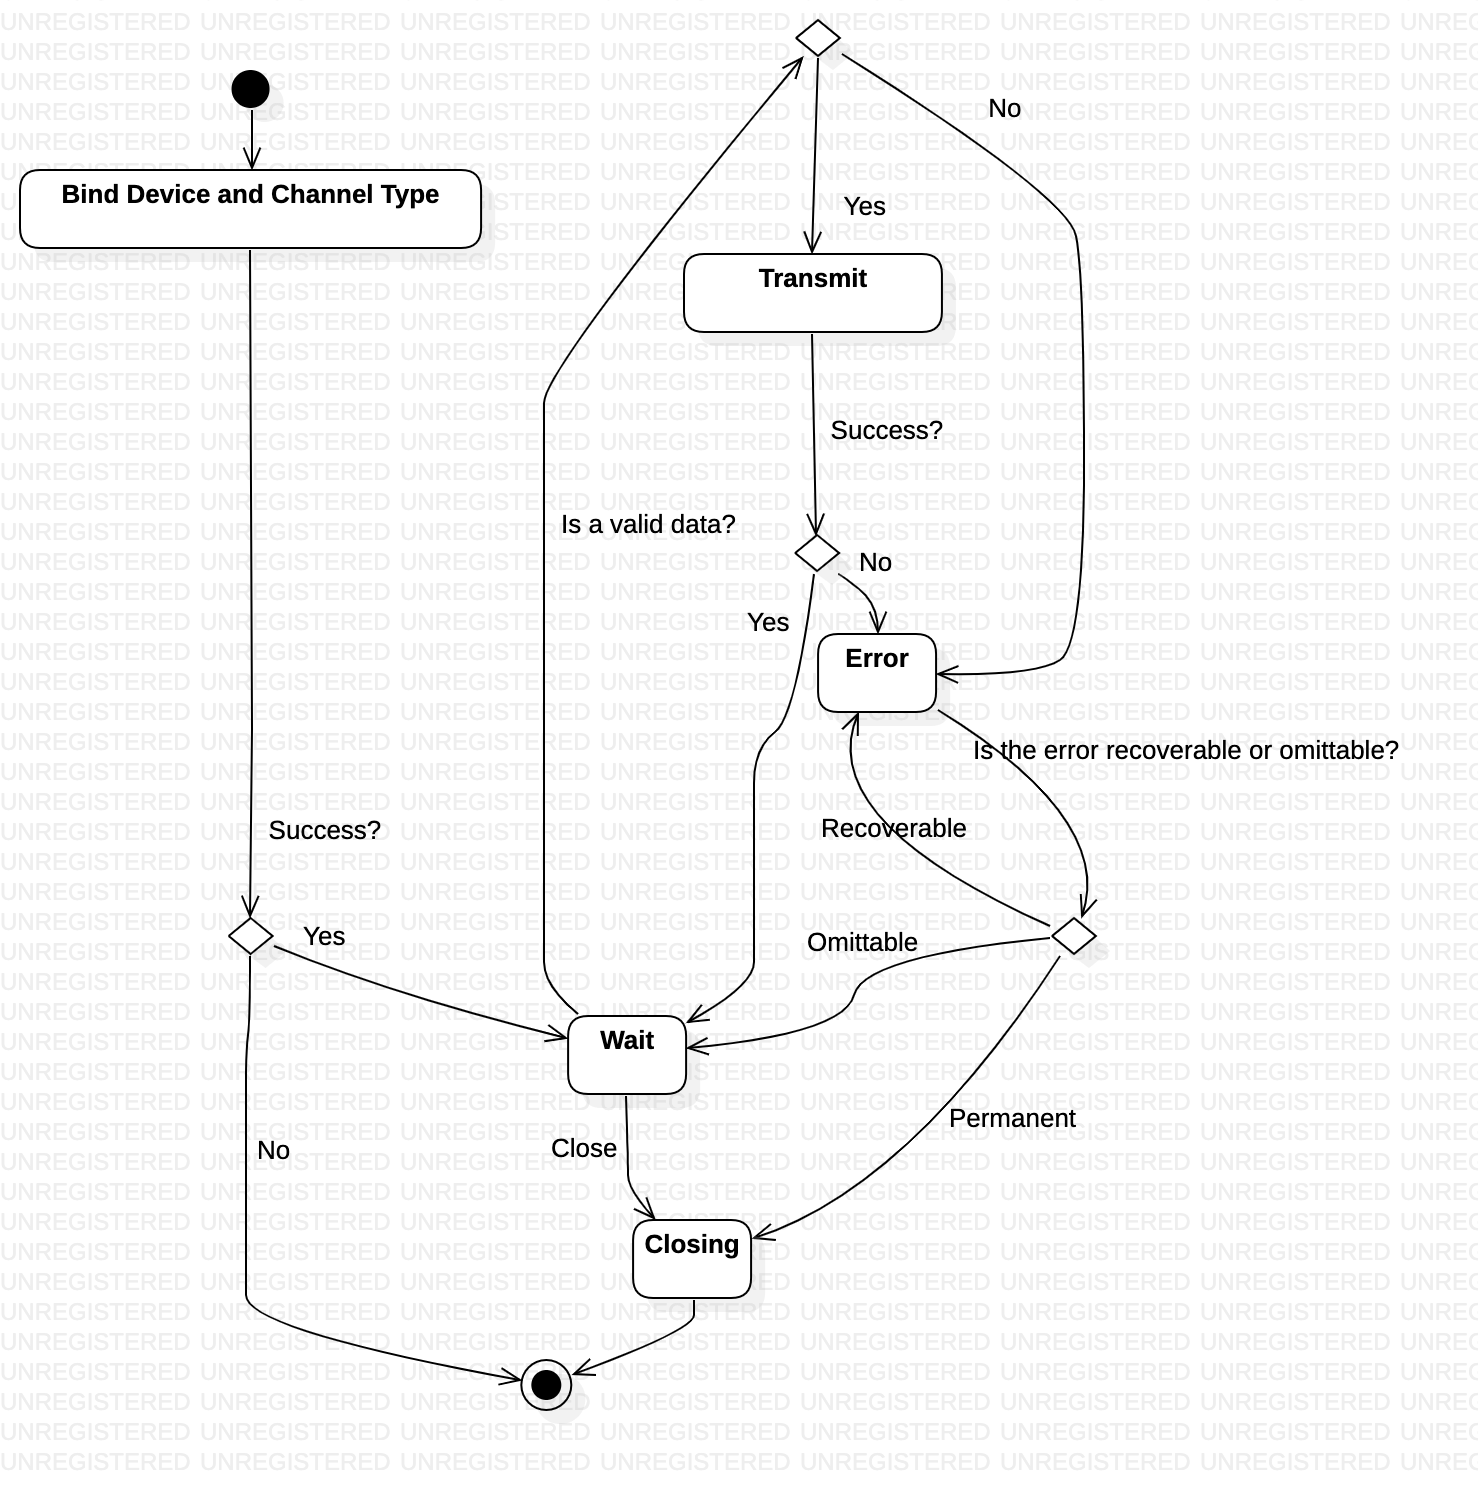
\includegraphics[width=16cm,height=16cm]{img/DR00012_BUS_statemachine.png}
\end{figure}
\newpage

\chapter{Transmission Task}
Generally, there are two direction of transmission, push and pull, and four types of tasks for each direction.\\
In push task, sender will send request to bus, and bus will set timer to start timing and send signal to check status of receiver. If receiver is available, bus will acknowledge sender, so that sender can start sending data.\\
In pull task, receiver will send request to bus, and bus will set timer to start timing and send signal to check status of sender. If sender is available, bus will acknowledge receiver, then sender can start receiving data.\\
Bus is possible requested by multiple devices. Then bus will decide which request should be process, basing on the availability of interruption of current task and priority of all related tasks. A lower priority and interruptible task will be interrupted by a higher priority task.\\
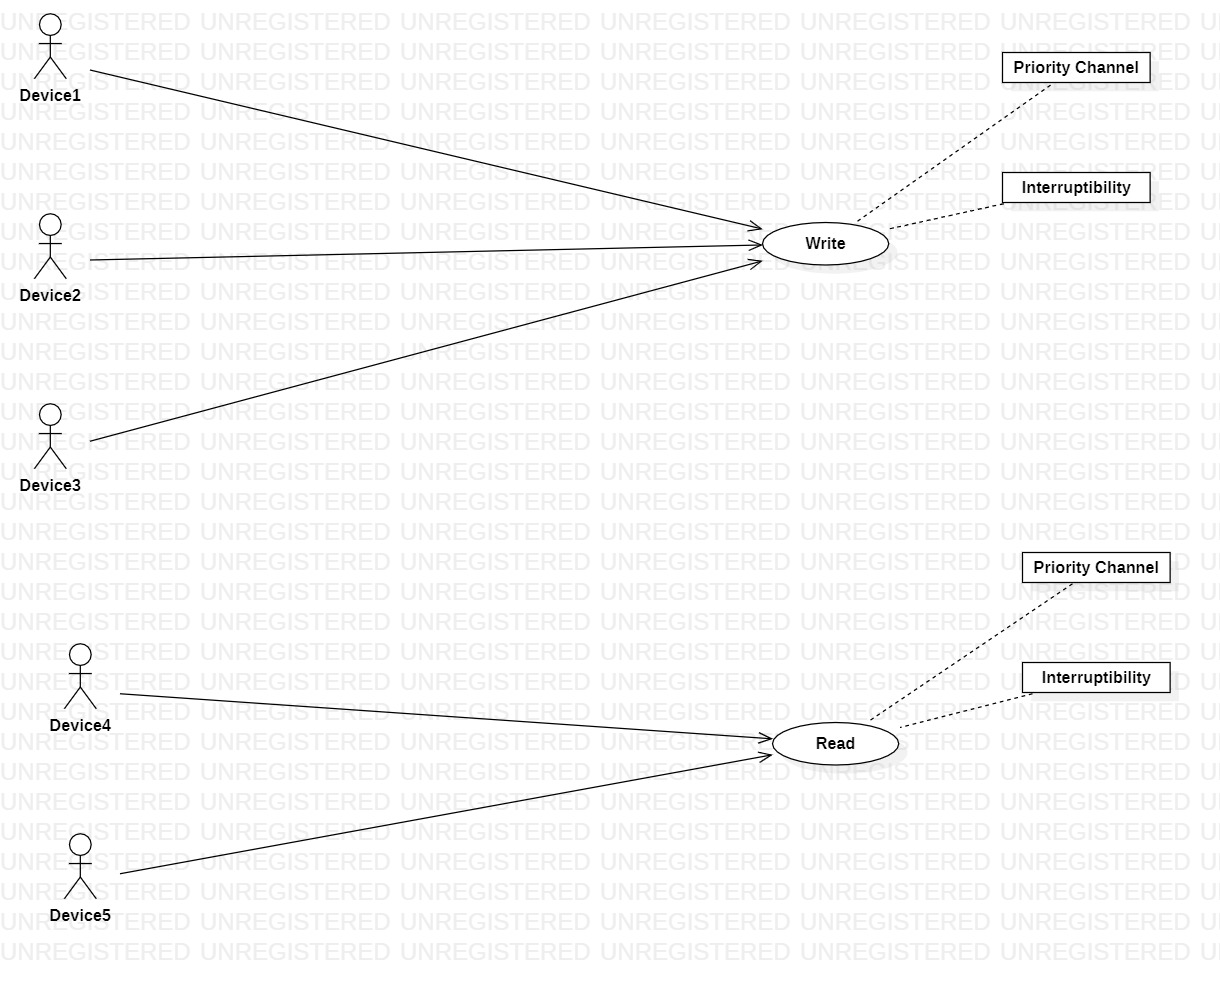
\includegraphics[width=8cm,height=8cm]{img/DR00012_Use_Case.jpg}

\newpage
\section{Acknowledge task}
When there is no need of perfect data accuracy, or there is a large amount of data need to be transferred. In this kind of task, there is no acknowledge after each data transmission, except the first time that bus will return the status of the target device.\\
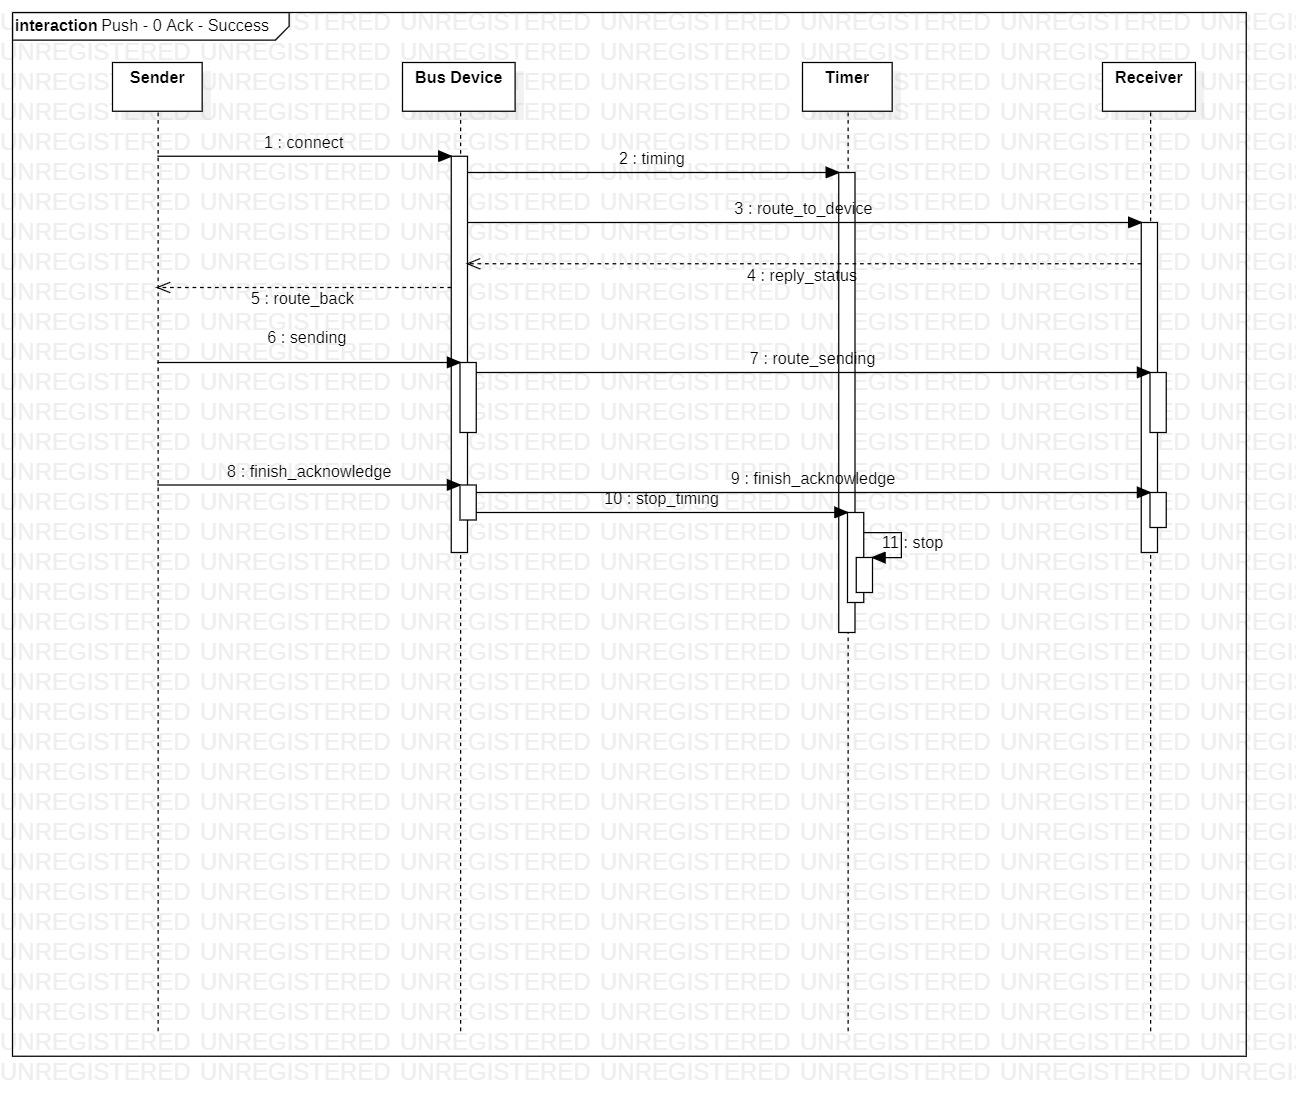
\includegraphics[width=8cm,height=8cm]{img/DR00012_Push_0_Ack_Success.jpg}
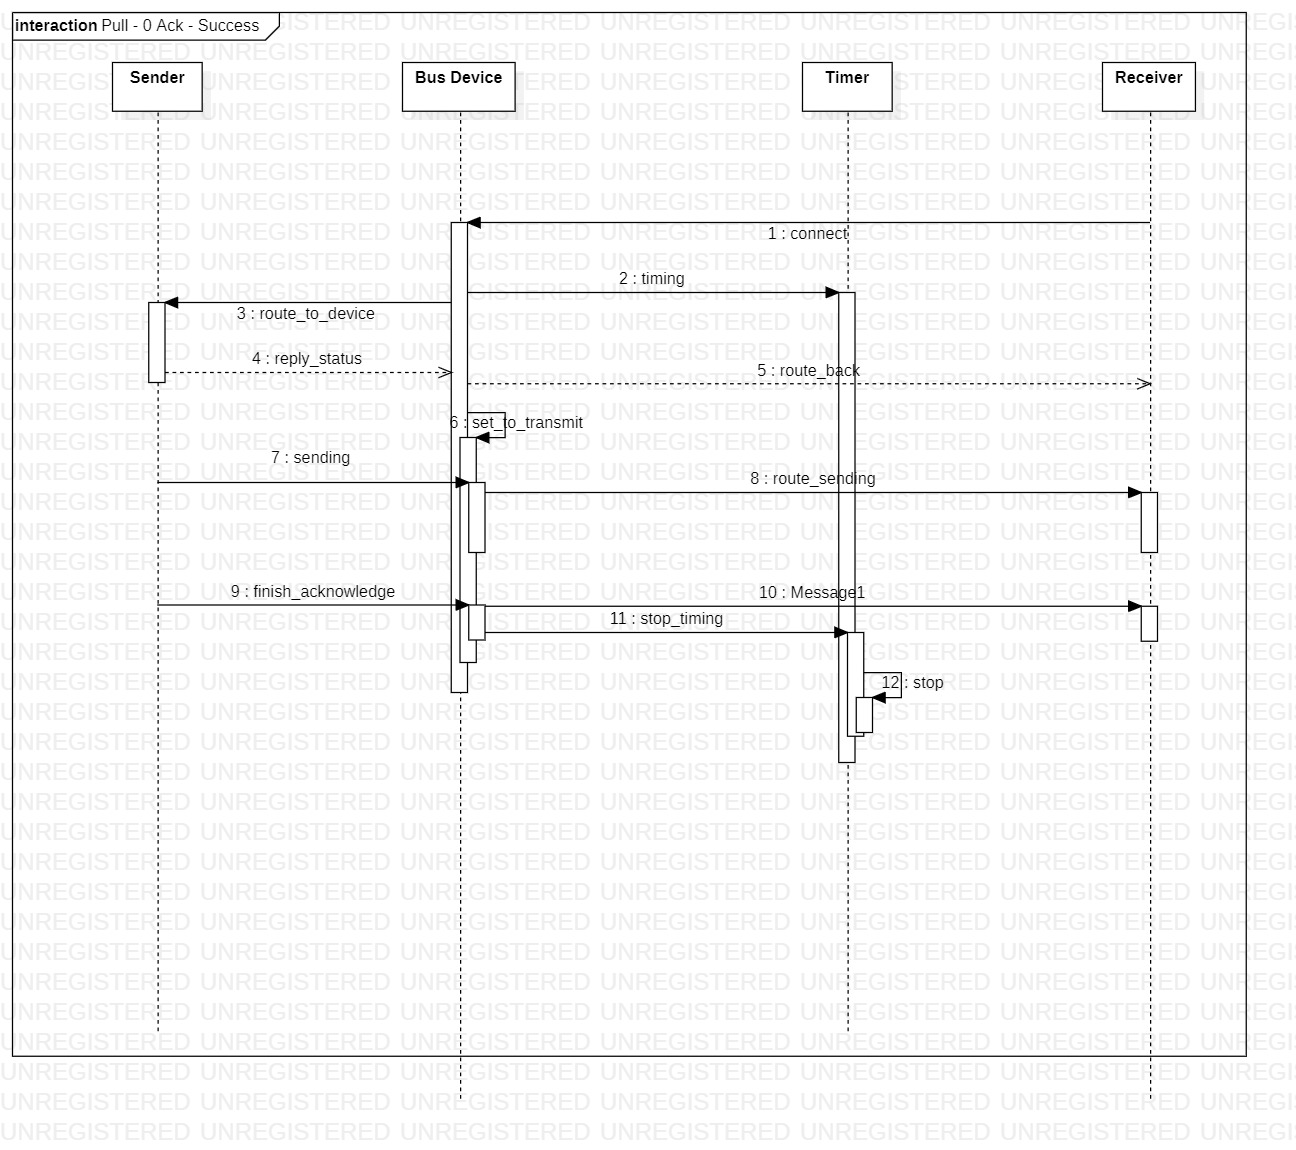
\includegraphics[width=8cm,height=8cm]{img/DR00012_Pull_0_Ack_Success.jpg}
\section{multi-acknowledge task}
All are the same as the 0 acknowledge task, except there will be a acknowledge after each data transmission to check the accuracy of data.\\
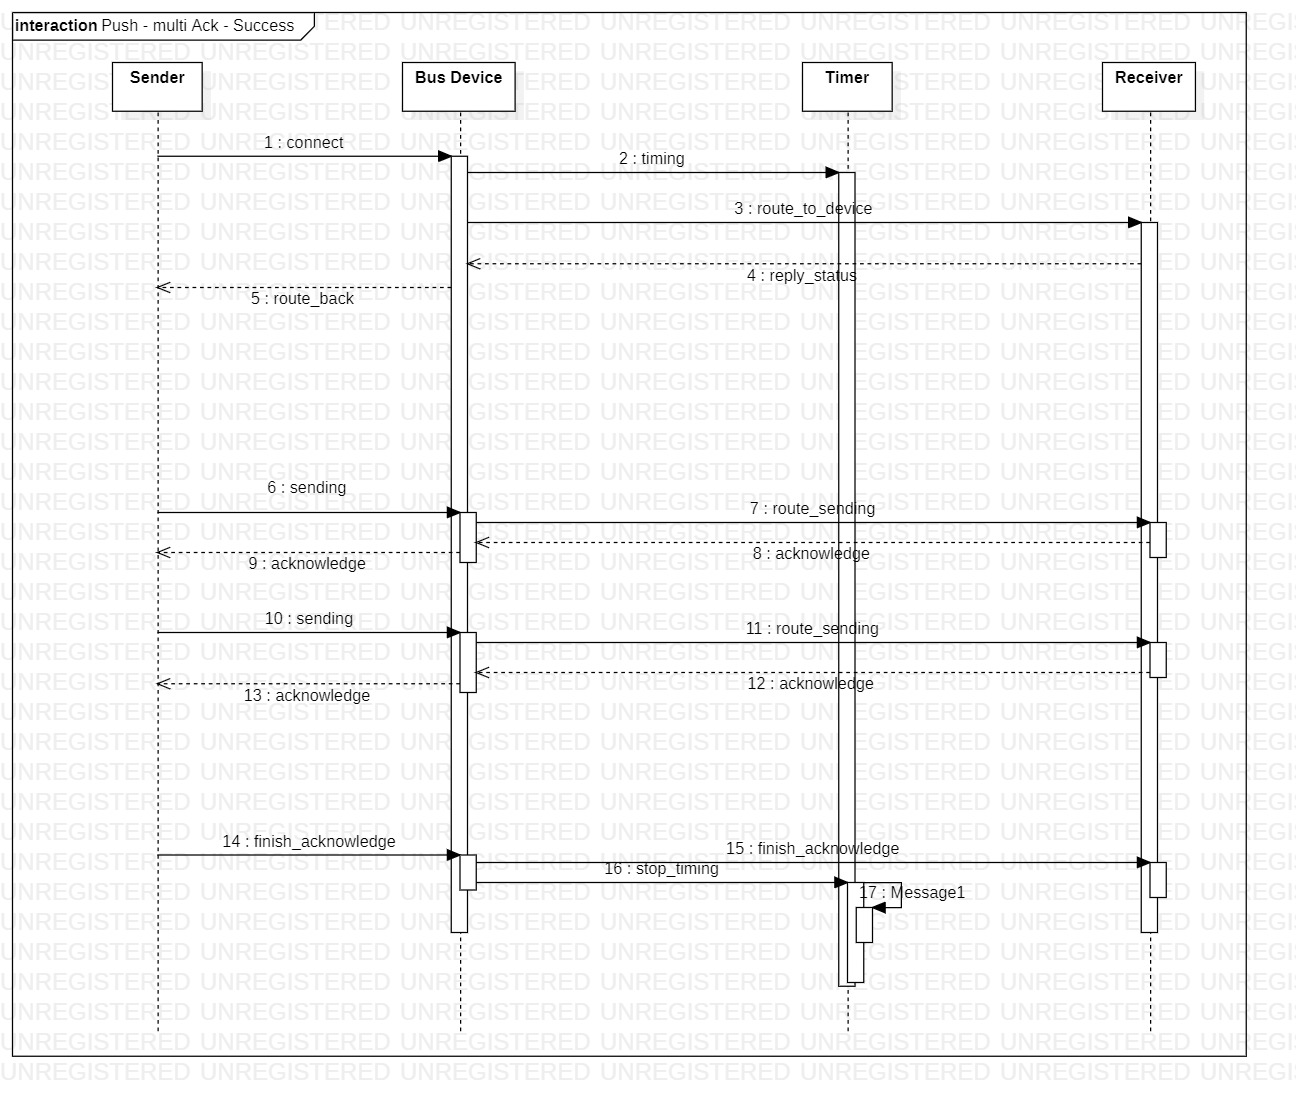
\includegraphics[width=8cm,height=8cm]{img/DR00012_Push_multi_Ack_Success.jpg}
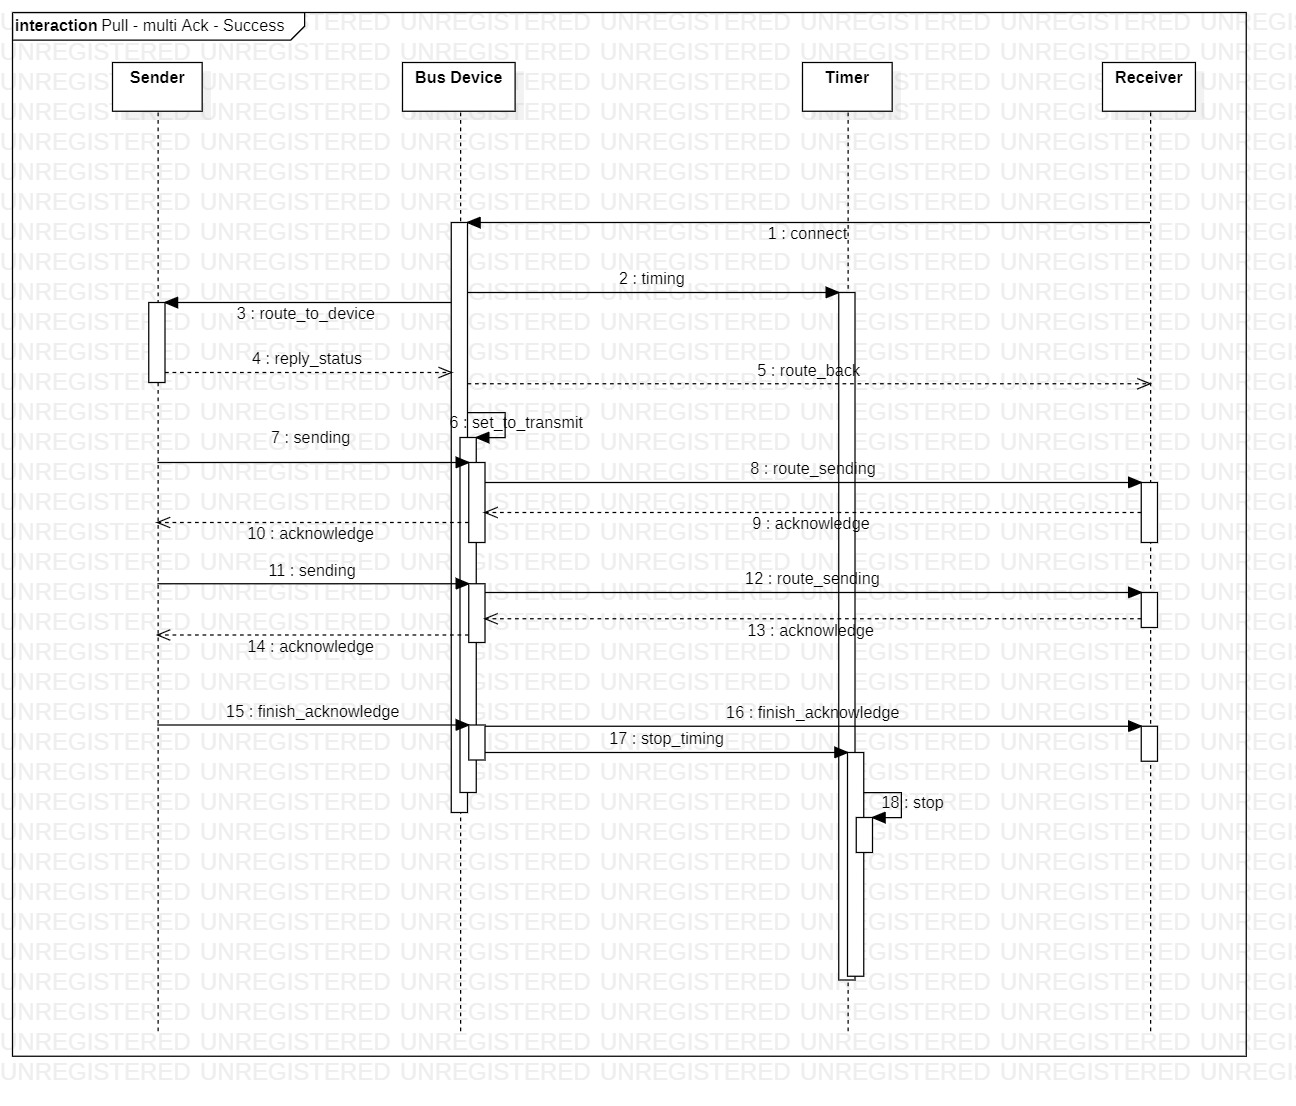
\includegraphics[width=8cm,height=8cm]{img/DR00012_Pull_multi_Ack_Success.jpg}
\section{Time out}
Both push and pull task start a timer at the beginning of the tasks. When the task duration is longer than the setted threshold, task will be terminated by bus.\\
In pull task, this could be results of target device no response or, simply, that the task duration is too long.\\
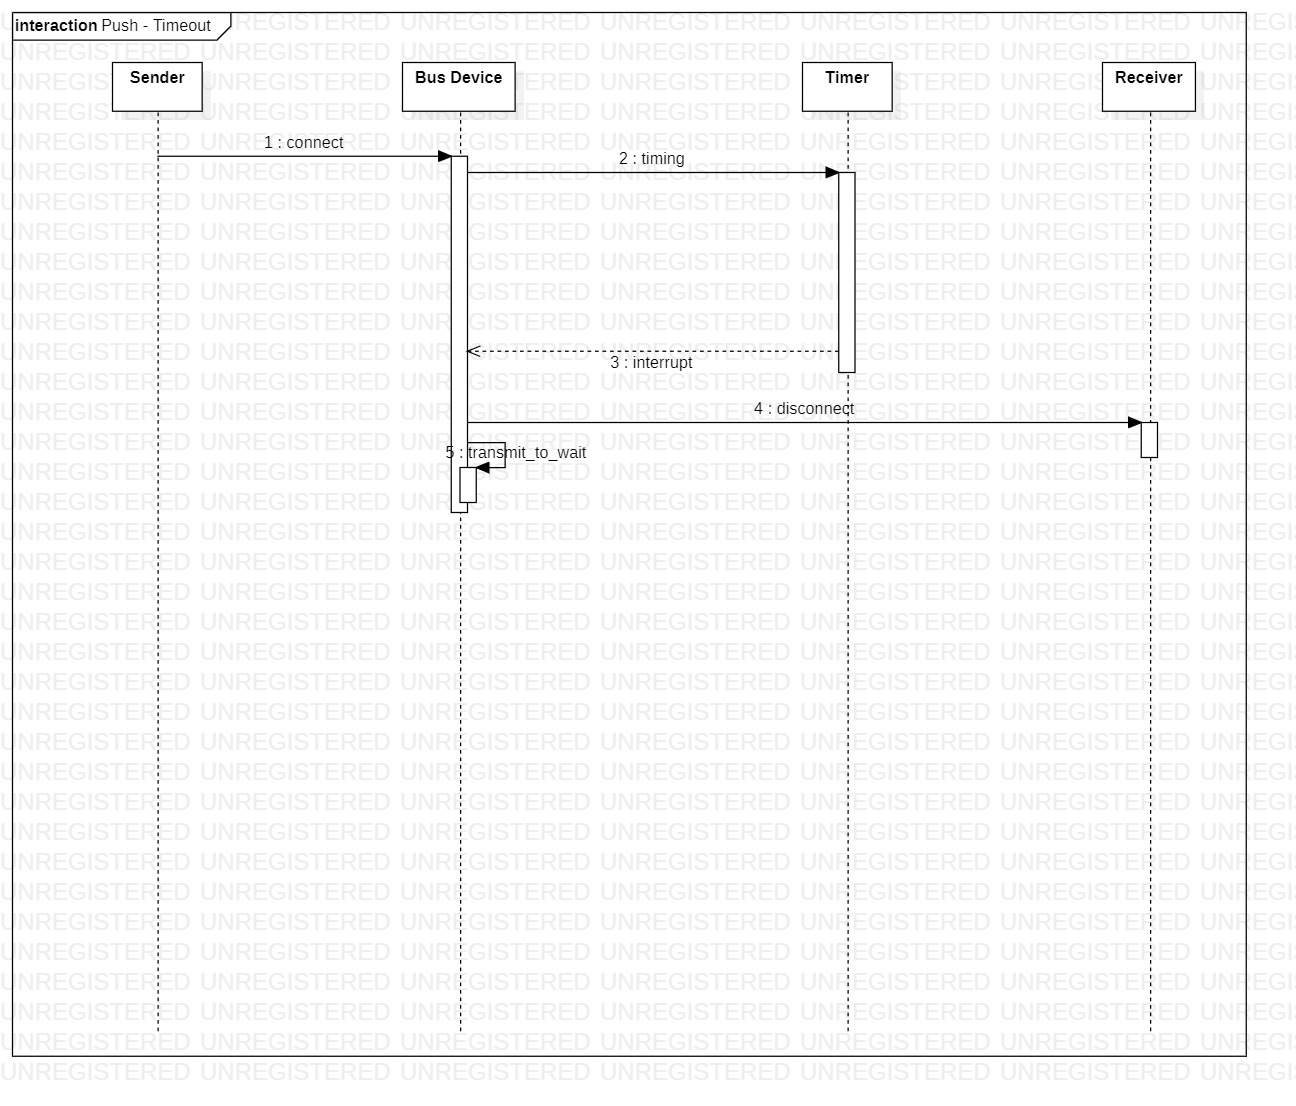
\includegraphics[width=8cm,height=8cm]{img/DR00012_Push_Timeout.jpg}
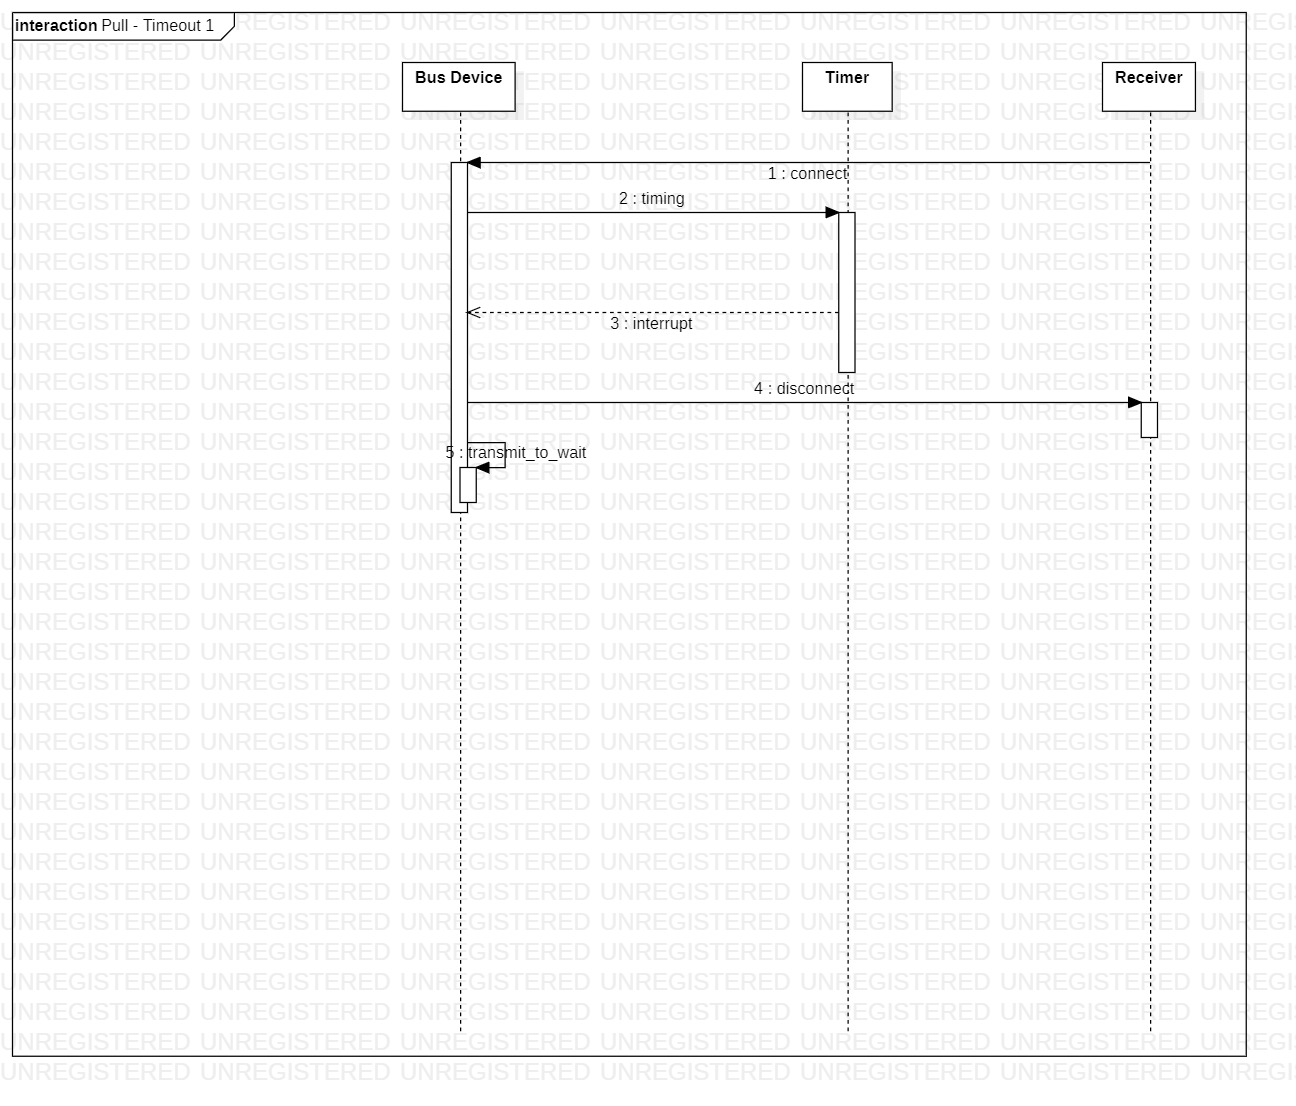
\includegraphics[width=8cm,height=8cm]{img/DR00012_Pull_Timeout_1.jpg}\\
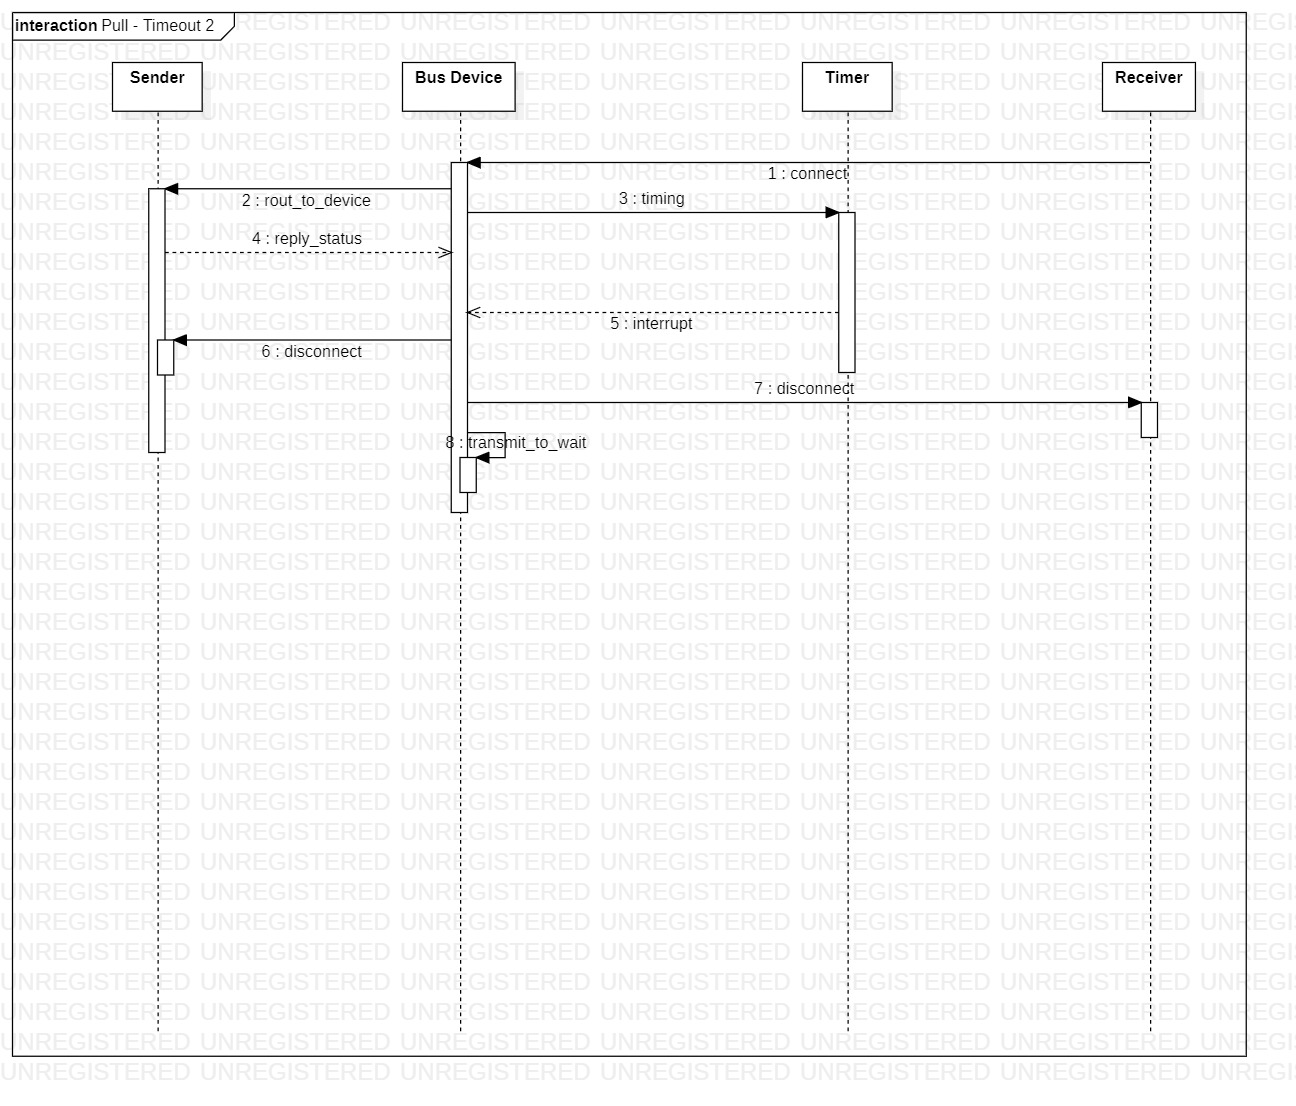
\includegraphics[width=8cm,height=8cm]{img/DR00012_Pull_Timeout_2.jpg}

\newpage
\section{Interruption}
This occurs when another higher priority request happens while a lower priority task is processing. Then the current task will be aborted, and bus will save space for prior task.\\
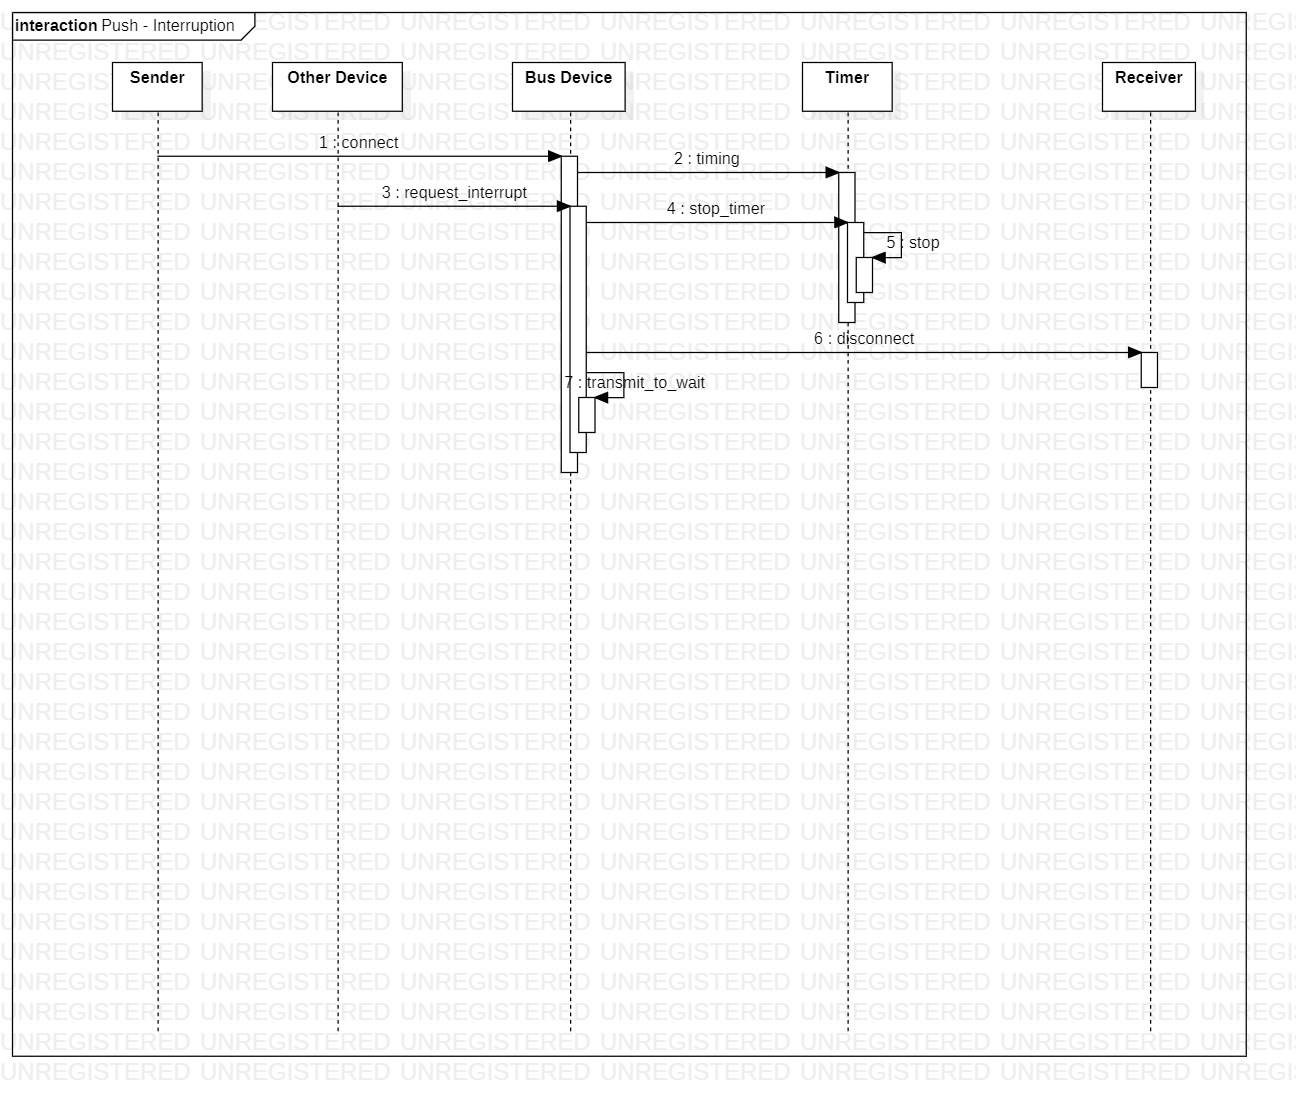
\includegraphics[width=8cm,height=8cm]{img/DR00012_Push_Interruption.jpg}
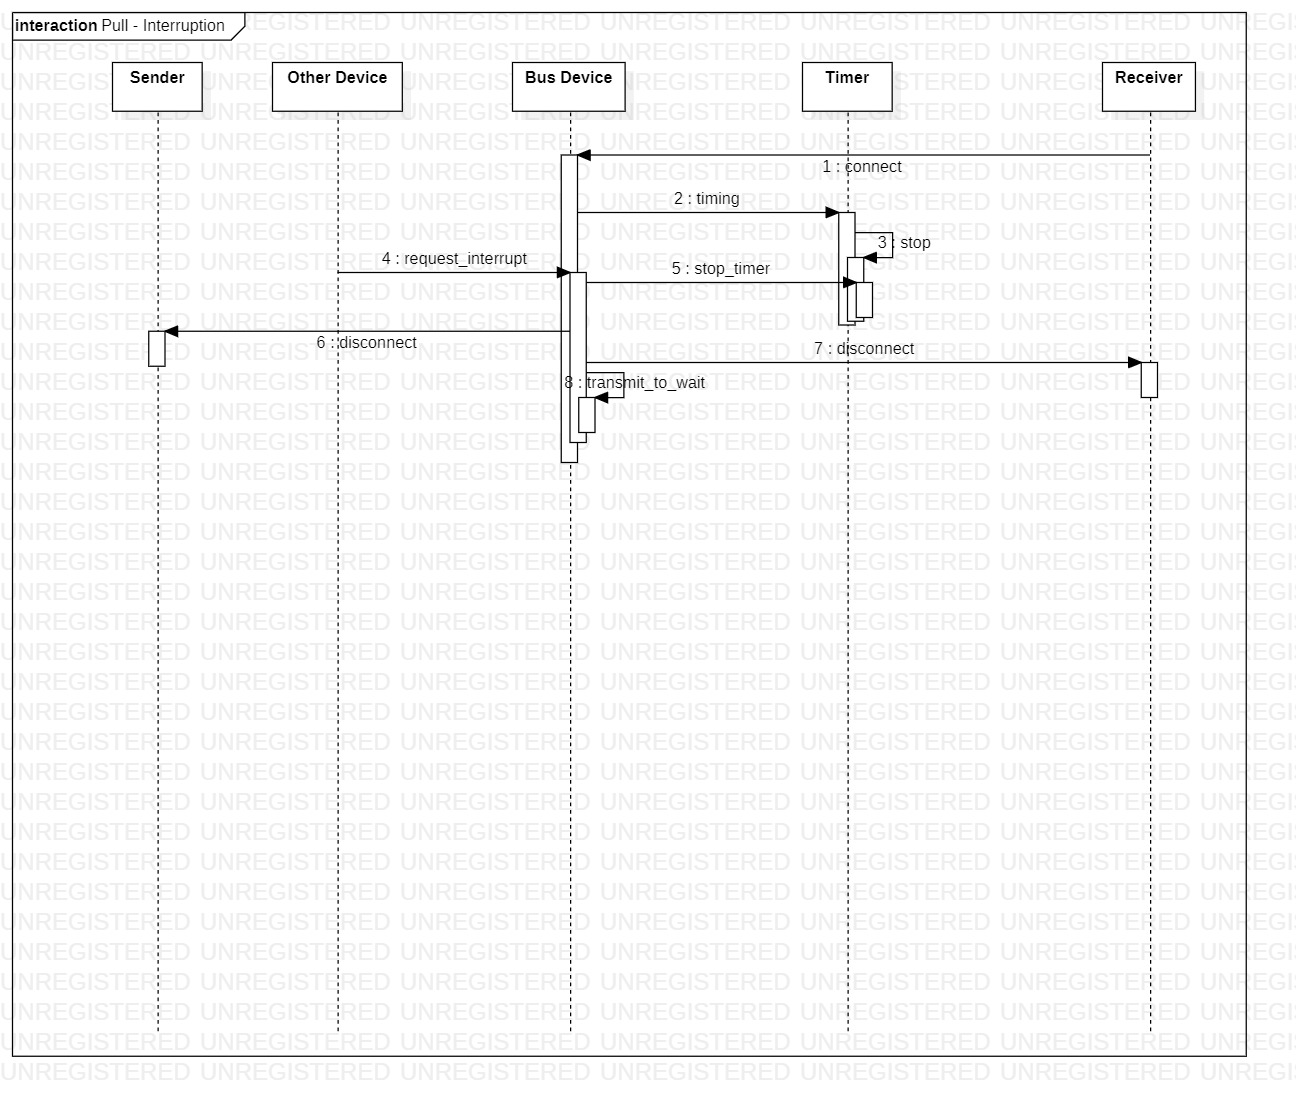
\includegraphics[width=8cm,height=8cm]{img/DR00012_Pull_Interruption.jpg}
\end{document}
% End of document
%**********************************************************************
